\documentclass[12pt]{article}
\usepackage{listings}
\usepackage{amsthm}
\usepackage[utf8]{inputenc}
\usepackage[english]{babel}
\usepackage{tikz}
\usetikzlibrary{arrows}
\usepackage{romande}
\usepackage[T1]{fontenc}
\usepackage{float}
\usepackage{url}
\usepackage{geometry}
\usepackage{marginnote}
\usepackage[autostyle]{csquotes}
\newtheorem*{definition}{Definition}
\theoremstyle{definition}
\newtheorem*{theorem}{Theorem}
\theoremstyle{theorem}

\lstdefinestyle{customc}{
	belowcaptionskip=1\baselineskip,
	breaklines=true,
	xleftmargin=\parindent,
    numbers=left,
    numberstyle=\ttfamily\color{gray},
	language=Java,
	showstringspaces=false,
	basicstyle=\footnotesize\ttfamily,
	keywordstyle=\bfseries\color{green!40!black},
	commentstyle=\itshape\color{purple!40!black},
	identifierstyle=\color{black},
	stringstyle=\color{orange},
}
\lstdefinestyle{customasm}{
	belowcaptionskip=1\baselineskip,
	frame=L,
	xleftmargin=\parindent,
	language=[x86masm]Assembler,
	basicstyle=\footnotesize\ttfamily,
	commentstyle=\itshape\color{purple!40!black},
}
\lstset{escapechar=@,style=customc}

\begin{document}
\begin{titlepage}
	\centering
    \null
    \vfill
    {\Large\itshape Comparing Testability and Usability in Software Paradigms
    \par}
    \vspace{3.0cm}
	{\scshape 
    A thesis presented \par 
    by\par
	Marc Coquand\par
	to\par
    The Department of Computer Science\par
    \vspace{0.8cm}
	for a degree of\par
    Master of Science in Engineering\par
    in the subject of\par
    Interaction Technology and Design\par}
    \vfill
    Umeå University\par
    Supervised by Anders Broberg\par
	\today\par
\end{titlepage}
\clearpage
\thispagestyle{empty}

\clearpage\newpage
\thispagestyle{empty}

\begin{abstract} 

    This study's goal is to compare approaches to functional programs and
    object-oriented programs to find how it affects maintainability and code
    quality. By looking at 3 cases, we analyze, how does a functional approach
    to software architecture compare to an OOP (Object-oriented programming)
    approach when it comes to maintainability and code quality? TO BE REPLACED
    WITH CONCLUSION

\end{abstract}

\clearpage\newpage
\thispagestyle{empty}

\section*{Acknowledgements}

I want to thank myself for my amazing work. TODO

\clearpage\newpage
\thispagestyle{empty}

\tableofcontents
\newpage

\section{Introduction}
This is time for all good men to come to the aid of their party! TODO

\section{Objective}

Different schools of thoughts have different approaches when it comes to
building applications. There is one that is the traditional, object oriented,
procedural way of doing it. Then there is a contender, a functional approach, as
an alternative way to build applications. When building applications testability
is of high concern to ensure that the application functions properly. By looking
at cyclomatic complexity, described in Section~\ref{cyclomaticcomplexity}, we
can find out how the different approaches affect the amount of tests we need to
write to get full branch coverage. By looking at the cognitive dimensions,
described in Section~\ref{cognitivedimensions}, we can find how the two
approaches affect the mental complexity for the developer. So by looking at
different case studies this study aims to find if the different software
paradigms affect the testability and if there are any cognitive benefits to one
approach over the other. 

\section{Theory}\label{theory}

\subsection{Characteristics of Functional Programming}

Functional programming is a software paradigm. While different definitions exist
of what it means, we define functional programming as:

\begin{itemize}
    \item Removing state to the outwards of the program
    \item Make functions pure, produce no side effects
    \item Using trait-based polymorphism rather than class-based
\end{itemize}

When a function is pure it means that calling a function with the same arguments
will always return the same value and that it does not mutate any value. For
example if you have $f(x) = 2\cdot x$, then $f(2)$ will always return $4$. It
follows then that an impure functions is either dependant on some state or
mutates state in some way. For example, given $g(x) = currenttime \cdot x$,
$g(5)$ will yield a different value depending on what time it is called. This
makes it dependant on some state of the world. Or given $x=0$, $h()=x+1$. Then
$h()$ will yield $x=1$ and $(h \circ h)()$ will yield $x=2$, making it
impure.~\cite{wikipedia_pure}

In OOP we inherit classes that contain methods and
attributes.~\cite{Gamma:1995:DPE:186897} For functional programs, we instead
define classes that describe the actions that are possible. For example, a class
\texttt{Equality} could contain a function \texttt{isEqual} that checks if two
data classes are equal. Then any data type that implements the interface
Equality, for example lists or binary trees, would be able to use the function
isEqual. This is known as type-classes in Haskell, mixins in Javascript or
Traits in Scala.

So while no exact definition of Functional programming exist, we here define it
as making functions pure and inheritance being based around functionality rather
then attributes.

\subsubsection{Structuring applications: interpreter pattern}

When structuring large functional applications there is no official way to do
it. For this study we will use a design pattern called the Interpreter pattern.
Informally, we can think of it as a way to create smaller composable compilers
that when added together make one big application. A compiler is a program that
takes some input, interprets the input and then does some output. A server, for
example, would take some request, interpret that request and then turn it into a
response. The server could integrate itself with the database, which would take
some query, interpret that query and then return an
object.~\cite{interpreterpattern}

To implement this pattern in Haskell we create an Abstract Syntax Tree (AST),
using a union type, of the program that contains all the available commands that
the program is capable of doing. See Figure~\ref{freeunion} for an example of a
to-do list AST. Once we have the AST we can encode the logic of the program as
instructions. Then the final step is to implement an interpreter for the program
that evaluates those commands. So if we have the commands in
Figure~\ref{freeunion}, we implement a function \texttt{eval} that takes a
command and computes some effectful code. The command \texttt{Add Item (Item ->
next)} could, for example, be executed as add an Item to the database.

\begin{figure}[H]
    \begin{lstlisting}
       data TodoList next
            = Add Item (Item -> next)
            | Mark Item next
            | Remove Item next
            | End --^ Terminates the program
    \end{lstlisting}
    \label{freeunion}
    \caption{AST for a to-do-list. We can derive a functor instances
    from ASTs for deriving Free instances.~\cite{commentarycompiler}}
\end{figure}


This allows us to separate effectful code (like output a string or send a http
request) with the logical instructions. This simplifies our testing, since we
can hide the environment (for example database) behind an interface that we can
swap out for testing. So we can implement two interpreter functions, one for our
real environment and one for testing. 

\subsubsection{Free Monads for interpreter pattern}

\marginnote{{\footnotesize\textbf{Note:} \textit{This part assumes familiarity
with Haskell and uninitiated can ignore it.}}}

If we implement an interpreter for an AST we will run into the Expression
problem. The expression problem states:

\blockquote{The goal is to define a data type by cases, where one can add new
cases to the data type and new functions over the data type, without recompiling
existing code, and while retaining static type safety.}

This means, if we try to add another operation to our AST we would have to add
new cases to every function using that data type. For small programs this is not
a problem but as this scales it could mean adding cases to thousands of
functions. 

To resolve this we will instance our to-do list as a Free Monad. A Free Monad is
a Monad that we get ``for free'' if we instance an AST as a Functor. With the
do-notation a Free Monad gives an interface we can use to write our program. So
we start off by instancing it as a Functor (example in
Figure~\ref{freefunctor}). This can also be derived automatically using the
DeriveFunctor extension.~\cite{commentarycompiler}.

\begin{figure}[H]
    \begin{lstlisting}
        instance Functor TodoList where
          fmap f (Add item k) = 
            Add item (f . k)
          fmap f (Mark item next) = 
            Set item (f next)
          fmap f End = 
            End
    \end{lstlisting}
    \label{freefunctor}
    \caption{A Functor instance for Figure~\ref{freeunion}. This can
    automatically be derived using DeriveFunctor.}
\end{figure}

From this we can define \texttt{type FreeAST = Free FunctorAst}. Lastly we lift
all the members of the union type as operations and create an interpreter. See
Figure~\cite{freeprogram} for a full example.

\begin{figure}[H]
    \begin{lstlisting}
        type TodoListF = Free TodoList

        add :: Item -> TodoListF Item
        add item = 
            liftF $ Add item id
        mark :: Item -> TodoListF ()
        mark item = 
            liftF $ Mark item ()
        end :: TodoListF r
        end = 
            liftF $ End

        eval :: TodoListF r -> IO r
        eval (Pure r) = return r
        eval (Free (Add item next)) = addItemToDb item >>= eval next
        eval (Free (Mark item next)) = markItem item >> eval next
        eval (Free End) = exitSuccess

        fakeItem :: Item

        exampleProgram :: TodoListF ()
        exampleProgram = 
            do  item <- add fakeItem 
                mark item 
                end

        main = 
            eval exampleProgram
    \end{lstlisting}
    \label{freeprogram}
    \caption{An example implementation for our To-do list data type defined in
    Figure~\ref{freeunion}.}
\end{figure}

So to summarize, if we just implement an evaluate function for our AST we run
into the expression problem. To mitigate this we use Free Monads to define our
ASTs and to get an interface that we can use with the do-notation. 

\subsection{Object Oriented Programming}\label{oop}

Object-oriented programming (OOP) is a programming paradigm based around the
idea of objects that contain attributes and methods. The general idea is that
you model the world through objects, where the programming objects represent the
objects in the real world. A shopping cart might have an object ``Customer'' and
an object ``Shopping list'', for example. Inheritance is also an important
concept in OOP, where one object can inherent methods and attributes of another
object.  For example, given an object Animal with the attributes health and the
method attack, another object Alligator could inherit those
properties.~\cite{Gamma:1995:DPE:186897}

\subsubsection{SOLID principles}

If the design of a system is done wrongly, it can lead to rotten design. Martin
Robert, a software engineer, claims that there are four big indicators of rotten
design.

First one is rigidity. Rigidity is the tendency for software to be difficult to
change. This makes it difficult to change non-critical parts of the software and
what can seem like a quick change takes a long time.

Second is fragility. Fragility is when the software tends to break when doing
simple changes. It makes the software difficult to maintain, with each fix
introducing new errors.

Third is immobility. Immobility is when it is impossible to reuse software from
other projects in the new project. So engineers discover that, even though they
need the same module that was in another project, too much work is required to
decouple and separate the desirable parts.

Last is viscosity. Viscosity comes in two forms: the viscosity of the
environment and the viscosity of the design. When the engineer makes changes
they are often met with multiple solutions. Some that preserve the design and
some that are ``hacks''. So the engineer can easily do the wrong thing.

When the compile times are long the engineers will attempt to make changes that
do not cause long compile times. This leads to viscosity in the environment.

To avoid creating rotten designs, Martin Robert proposes the SOLID guidelines.
SOLID mnemonic for five design principles to make software more maintainable,
flexible and understandable. The SOLID guidelines are

\begin{itemize}
    \item Single responsibility principle. Here, responsibility means ``reason
        to change''. Modules and classes should have one reason to change and no
        more.
    \item Open/Closed principle. States we should write our modules to be
        extended without modification of the original source code.
    \item Liskov substitution principle. Given a base class and an derived
        class derive, the user of a base class should be able to use the derived
        class and the program should function properly.
    \item Interface segregation principle. No client should be forced to depend
        on methods it does not use. The general idea is that you want to split
        big interfaces to smaller, specific ones.
    \item Dependency inversion principle. A strategy to avoid making our source
        code dependent on specific implementations is by using this principle.
        This allows us, if we depend on one third-party module, to swap that
        module for another one should we need to. This can be done by creating
        an abstract interface and then instance that interface with a class that
        calls the third-party operations.~\cite{martinrobert}
\end{itemize}

When we compare our solutions we want to test them after principles used in the
industry, as then we can use the results when making technical decisions for our
softwares.

\section{Methods}\label{methods}

\subsection{Measuring testability: Cyclomatic Complexity}\label{cyclomaticcomplexity}

Cyclomatic complexity is a complexity measure that allows us to measure the
amount of paths through a program. The Cyclomatic complexity number is an upper
bound for the number of test cases required for full branch coverage of the
code. 

\theoremstyle{definition}
\begin{definition}
The cyclomatic number $v(G)$ of a graph G with $n$ vertices, $e$ edges and $p$
connected components is $v(G) = e - n + p$.
\end{definition}

\begin{theorem}
In a strongly connected graph $G$, the cyclomatic number is equal to the
maximum number of linearly independent circuits.~\cite{McCabe}
\end{theorem}

Informally, we can think of cyclomatic complexity as a way to measure the amount
tests a program needs to reach full branch coverage. We construct a graph that
branches out based on when the control flow in our source code branches out. For
example, given \texttt{f(bool) = if bool then 1; else 2}, the function
\texttt{f} will either be 1 or 2. The function \texttt{f} will need two tests in
order to have full code coverage. The cyclomatic complexity in this case is 2.
The nodes of the graph represents processing tasks and edges represent control
flow between the nodes. 

\begin{figure}[H]
    \begin{lstlisting}
        void foo(void)
        {
          if (a)
            if (b) 
              x=1;
          else
              x=2;
         }
    \end{lstlisting}
    \caption{Multi if function foo.}\label{c1excode}
\end{figure}

If we have the code found in example figure~\ref{c1excode}. To calculate the
complexity of this function we first construct a graph as seen in
figure~\ref{fig:c1exgraph}. From the graph we find $n=4, e=5, p=2\Rightarrow
v(G)=e-n+p=5-4+2=3$ is the cyclomatic number.

\begin{figure}[H]
    \centering
    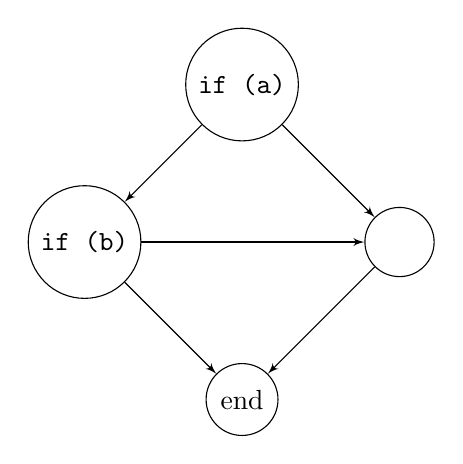
\begin{tikzpicture}
        \tikzset{vertex/.style = {shape=circle,draw,minimum size=2.5em}};
        \tikzset{edge/.style = {->,> = latex'}};
        \node[vertex] (a) at (2,8) {\texttt{if (a)}};
        \node[vertex] (b) at (0,6) {\texttt{if (b)}};
        \node[vertex] (c) at (4,6) {};
        \node[vertex] (d) at (2,4) {end};
        \draw[edge] (a)  to (b);
        \draw[edge] (a)  to (c);
        \draw[edge] (b)  to (c);
        \draw[edge] (b)  to (d);
        \draw[edge] (c)  to (d);
    \end{tikzpicture}
    \caption{Cyclomatic complexity graph for Figure~\ref{c1excode}}\label{fig:c1exgraph}
\end{figure}

\subsubsection{Cyclomatic Complexity in Functional Programming}

The definition of cyclomatic complexity in Section~\ref{cyclomaticcomplexity} is
not ideal for functional programming. Cyclomatic complexity is calculated by
creating graphs based on control flow operations such as while loops and if
statements. In functional programming everything is a function, thus the
cyclomatic complexity will always tend to 0 using this definition. So we define
a different method of calculating the cyclomatic complexity for functional
programs. 

\theoremstyle{definition} 
    \begin{definition} 
    The cyclomatic complexity number, in functional programming, is equal to
    1 plus the sum of the left hand side, called LHS, plus the sum of the
    right hand side, called RHS. RHS is the sum of the number of guards,
    logical operators, filters in a list comprehension and the pattern
    complexity in a list comprehension. LHS is equal to the pattern
    complexity.  The pattern complexity is equal to the number of
    identifiers in the pattern, minus the number of unique identifiers in
    the pattern plus the number of arguments that are not identifiers. In
    summary:

    \begin{lstlisting}
    Cyclomatic complexity = 1 + LHS + RHS

    LHS = Pattern complexity 

    Pattern complexity   
        = Pattern identifiers 
        - Unique pattern identifiers 
        + Number of arguments that are non identifiers

    RHS = Number of guards 
        + Number of Logical operators 
        + Number of filters in list comprehension 
        + Pattern complexity in list comprehension
    \end{lstlisting}
\end{definition}

Instead of cyclomatic graphs we instead construct flowgraphs, such as the one
seen in Figure~\ref{fig:cyclomaticfunctional} to model our function.

\begin{figure}[H]
    \begin{lstlisting}
    split :: (a -> Bool) -> [a] -> ([a], [a])
    split onCondition [] = ([], [])
    split onCondition (x:xs) =
        let 
            (ys, zs) = split onCondition xs
        in 
            if (onCondition x) then 
                (x:ys, zs)
            else 
                (ys, x:zs)
    \end{lstlisting}
    \label{split}
    \caption{Recursively split a list into two based on a given condition in
    Haskell. For example \texttt{split (>3) [1,2,3,4,5] =
    ([4,5],[1,2,3])}.}
\end{figure}

In Haskell $(x:xs)$ denotes an item $x$ at head of a list of items $xs$. Given
the Haskell code in Figure~\ref{split}. To calculate LHS we find two
pattern identifiers which are $onCondition$ and $(x:xs)$. there is one unique
pattern identifiers which is $(x:xs)$. There is also one non identifier
which is $[]$. We also find one guard, an if statement, and no
list comprehensions on RHS. Thus the cyclomatic complexity is $1+(2-1+1)+1=4$.
<-- NEEDS VERIFICATION FROM SOMEONE, THE SOURCE IS VERY VAGUE HERE\ldots

We do not count the $otherwise$ and $else$ clauses as a guard, just as how we
do not count the $else$ statement in normal procedural cyclomatic
complexity.~\cite{bergklaas}


\begin{figure}[H]
    \centering
    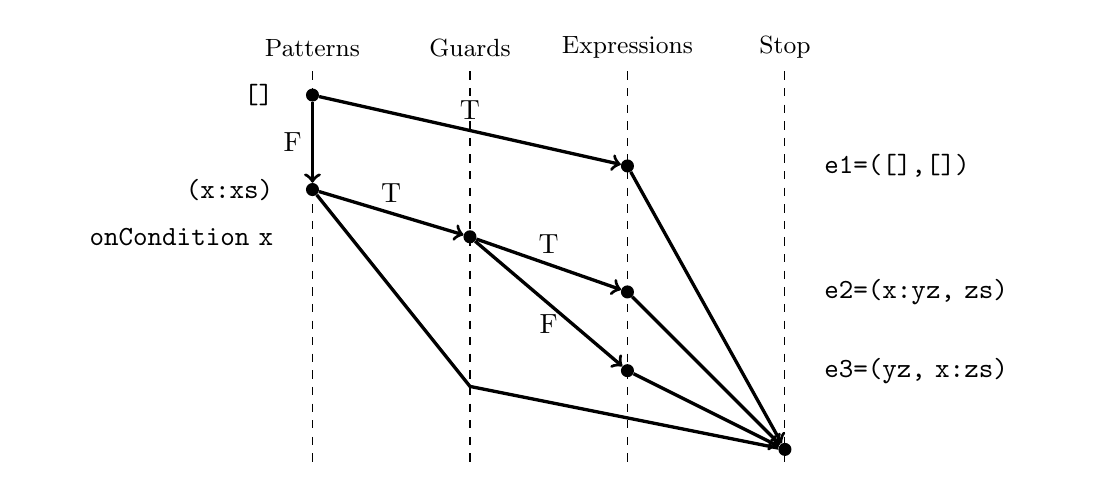
\begin{tikzpicture}
        \tikzset{vertex/.style = {shape=circle,fill=black,scale=0.5}};
        \draw[dashed] (0,0) -- (0,-5) (2,0) -- (2,-5) (4, 0) -- (4, -5) (6, 0)
        -- (6, -5);
        \node at (0,.3) {\small{Patterns}};
        \node at (2,.3) {\small{Guards}};
        \node at (4,.3) {\small{Expressions}};
        \node at (6,.3) {\small{Stop}};
        \node[vertex] (a) at (0,-0.3) {};
        \node[align=right, text width=3cm] at (-2,-0.3) {\texttt{[]}};
        \node[vertex] (b) at (4,-1.2) {};
        \draw[->, very thick] (a) to node [above] (TextNode) {T} (b) ;
        \node[vertex] (c) at (0,-1.5) {};
        \node[align=right, text width=3cm] at (-2,-1.5) {\texttt{(x:xs)}};
        \draw[->, very thick] (a) to node [left] (TextNode) {F} (c) ;
        \node[align=left, text width=3cm] at (8,-1.2) {\texttt{e1=([],[])}};
        \node[vertex] (d) at (2,-2.1) {};
        \draw[->, very thick] (c) to node [above] (TextNode) {T} (d) ;
        \node[align=right, text width=3cm] at (-2,-2.1) {\texttt{onCondition x}};
        \node[vertex] (e) at (4,-2.8) {};
        \draw[->, very thick] (d) to node [above] (TextNode) {T} (e) ;
        \node[align=left, text width=3cm] at (8,-2.8) {\texttt{e2=(x:yz, zs)}};
        \node[vertex] (f) at (4,-3.8) {};
        \draw[->, very thick] (d) to node [below] (TextNode) {F} (f) ;
        \node[align=left, text width=3cm] at (8,-3.8) {\texttt{e3=(yz, x:zs)}};
        \node[vertex] (g) at (6,-4.8) {};
        \draw[->, very thick] (e) to (g) ;
        \draw[->, very thick] (b) to (g) ;
        \draw[->, very thick] (f) to (g) ;
        \draw[very thick] (c) to (2, -4.0) to (g) ;
    \end{tikzpicture}
    \label{fig:cyclomaticfunctional}
    \caption{Flowgraph for split function, defined in Figure~\ref{split}.}
\end{figure}

\subsection{Mental complexity: Cognitive Dimensions}\label{cognitivedimensions}

Cognitive Dimensions is a framework for evaluating the usability of programming
languages and to find areas of improvements. Used as an approach to analyse the
quality of a design, it also allows to explore what future designs could be
possible. As part of the Cognitive Dimensions, 14 different Cognitive Dimensions
of Notation exist. A notation depends on the specific context, in this case will
be the languages themselves and their architecture.

\subsubsection{Viscosity}

How much work does it take to make small changes? How easy is the code to
refactor? If small changes requires consequent adjustments then that is a
problem. As a viscous system cause a lot more work for the user and break the
line of thought.

\subsubsection{Visibility}

How easy is it to navigate the source code to find the parts that you want?

\subsubsection{Premature Commitment}

Are there any architectural decisions that must be made before all the necessary
decisions have been made? Can we correct those decisions later, how safe is the
refactoring and how much is needed? If you imagine a word processor which
required how many pages of text would be used before being written then
that would be premature commitment.

\subsubsection{Hidden Dependencies}

Are there hidden dependencies in the source code. Does a change in one part of
the source code lead to unexpected consequences in another part of the code.
Every dependency that matters to the user should be accessible in both
directions. 

\subsubsection{Role-Expressiveness}

How obvious is each sub-component of the source code to the solution as a whole?

\subsubsection{Abstraction}

What are the levels of abstraction in the source code? Can the details be
encapsulated?

\subsubsection{Secondary Notation}

Are there any extra information being conveyed to the user in the source code?

\subsubsection{Closeness of Mapping}

By looking at the source code, how close do we find it to be to the case
we are solving?

\subsubsection{Consistency}

Once Object-oriented procedural programming and Functional programming has been
learned. How much of the rest can the user guess successfully? 

\subsubsection{Diffuseness or terseness}

How much space and symbols does the source code need to produce a certain result
or express a meaning?

\subsubsection{Hard Mental Operations}

Where does the hard mental processing lie? Is it more when writing the source
code itself rather than solving the case, I.E. the semantic level? Do you
sometimes need to resort to pen and paper to keep track of what is happening?

\subsubsection{Provisionality}

How easy is it to get feedback of something before you have completed the entire
system?

\subsubsection{Progressive Evaluation}

How obvious the role of each component of the source code in the solution as a
whole?~\cite{GREEN1996131}

\subsection{Case studies}

To compare the different paradigms using Cognitive dimensions and measuring
Cyclocmatic complexity we will look at three different cases. The cases were
chosen based on how they are often subproblems in bigger applications.

\subsubsection{Simplified chess game}

Chess is a famous game and assumed that the reader know how it works. Aim
is to implement a simplified variant of it. This is not ordinary chess but a
simplified version:

\begin{itemize} 
    \item Only pawns and horses exist.
    \item You win by removing all the other players pieces.
\end{itemize}

The player should be able to do the following:

\begin{itemize} 
    \item List all available moves for a certain chess piece. 
    \item Move the chess piece to a given space
    \item Switch player after move
    \item Get an overview of the board
    \item Get an error when making invalid moves
\end{itemize}

To interact with the game, a user types commands through a command line prompt.
An example of basic interaction with the game is displayed in
Figure~\ref{chessexample}.

\begin{figure}[H]
    \centering
    \begin{lstlisting}
        > list (a,2)
        White pawn at (a,2)
        > move (a,2) (a,3)
        White pawn moved to (a,3)
        > listall
        White pawn at (a,3)
        White pawn at (b,2)
        ...
        White Horse at (a,1)
        ...
        Black pawn at (a,8)
        ...
    \end{lstlisting}
    \label{chessexample}
    \caption{An example of the interaction in the chess game.}
\end{figure}


\subsubsection{to-do List}

A common task in programming is to create some kind of data store with
information. A to-do list is a minimal example of that. It consists of a list of
items that can be used to remember what to do later. The user should be able to:

\begin{itemize}
    \item Create a new item in the to-do list.
    \item Remove an item from the to-do list.
    \item Mark an item from the to-do list as done.
    \item See all items in the to-do list.
\end{itemize}

The interface to this program will be a text interface, displaying each item in
the todo list. To navigate and mark an item in the list the user presses up and
down and presses \texttt{x} to mark it.

\subsubsection{Chatbot engine}

Oftentimes when developing applications we have to deal with complex information
input. One of those cases is when we have chat bots. Chat bots are interactive
programs that respond with a text answer to the users input. For this
application we will implement the following:

\begin{itemize}
    \item Interpretor that can handle semi-complex inputs and deal with errors.
    \item Give answers to those inputs in form of text messages.
\end{itemize}    

\section{Results}\label{results}
We worked so hard, yet achieved very little. TODO

\section{Limitations}\label{limitations}

TODO

\subsection{Improvements to implementation}
TODO

\section{future work}
\subsection{Relations to cardinality}
TODO

\bibliographystyle{ieeetr}
\bibliography{thesis}

\end{document}
